\chapter{Environment Setup} \label{chapter:environment}
As we have mentioned before, ideally the project's environment would be a physical network with OpenFlow switches. Since that is not possible for us, we will set up a virtual environment using a Mininet virtual machine. Consequently, this chapter will walk us through the process of setting up the virtual machine as well as the creating the network topology.

\section{Mininet Virtual Machine}
As a reminder, a virtual machine is not strictly necessary, as it can be installed natively in an already existing GNU/Linux system. Nonetheless, virtualization has a few advantages:
\begin{itemize}
    \item \textbf{Custom Linux kernel}. The Mininet virtual machine includes a custom Linux kernel optimized towards network virtualization.
    \item \textbf{Isolation}. It allows us to work on an isolated environment, so that the host system does not interfere. In essence, we have a simplified system that is easier to troubleshoot in the event that something goes wrong.
    \item \textbf{Repeatability}. We can reproduce the environment in different machine without having to reconfigure everything from scratch.
\end{itemize}

On the other hand, using a virtual machine also comes with some disadvantages such as extra overhead and networking becomes slightly trickier.

With that said, the very first thing we need to do is download the image file, which can be found here \url{https://github.com/mininet/mininet/wiki/Mininet-VM-Images}. There are several images to choose from, although most of them are deprecated old versions. Since we are running GNU/Linux as the host system, we have chosen "Mininet 2.2.2 on Ubuntu 14.04 LTS - 64 bit", which is the latest version at the time of writing this document.

Next up, after the download and decompressing the file, we are left with two files with the extensions ".ovf" and ".vmdk". The easiest way to proceed is to import the image using the ".ovf" file. If, for some reason, the import fails, we can manually create a new virtual machine and use the ".vmdk" file as hard disk.

After importing the image, we can now launch it and log in. The default credentials for username and password are mininet and mininet respectively. When we log in, we will notice that image does not include a display renderer, i.e., we do not have a graphical environment. From here we have three options.
\begin{enumerate}
    \item Work without a graphical environment and within the native Virtual Box terminal. The easiest option, does not require any extra configuration but it is also very limited and cumbersome. This option would not allow us to use graphical applications such as Wireshark.
    
    \item Install a display renderer and desktop environment or window manager. This requires quite a lot of extra memory usage within the virtual machine as well as overhead. In spite of having a worse performance, it is the most user friendly option.
    
    \item SSH into the virtual machine and work from the host machine using X forwarding. Very little overhead but it requires some configuration for it to work properly. This option is only possible if the host machine is running a Xorg server (display renderer).
\end{enumerate}

We will stick to option three since it is the one we feel the most comfortable and our host meets the requirements. In order to do it this way, we have to do the following.
\begin{enumerate}
    \item In the virtual machine, make sure at least one network adapter enabled either in host-only or bridge mode. For the latter, ensure the host is already connected to a network.
    
    \item Find out the IP address of the network adapter we just enabled. If there are several network adapters enabled, it is possible that the one we are interested on does not have an IP address assigned to it. If that is the case, use the \textit{dhclient} command manually.
    
    \item Connect to the virtual machine using the following command.
    \begin{lstlisting}
        ssh -Y mininet@<IP Address>
    \end{lstlisting}
    
    The -Y flag stands for trusted X forwarding. Regular X forwarding has a 20 minutes timeout and causes some issues when using Xterm within Mininet. Note that trusted X forwarding should not be used lightly and could have security implications.
    
    \item (Optional). Generate a private and public key pair on the host and transfer the public key to the virtual machine under \\ /home/mininet/.ssh/authorized\_keys. This will allow us to log into the machine without having to type the password every time.
\end{enumerate}

Finally, in preparation for the testing phase, we need to enable two additional network adapters on bridge mode. We will use these adapters to connect two external physical hosts to the Mininet network. After all of this, we are done configuring the virtual machine itself. We are ready to start setting up the Mininet topology.

\section{Mininet}
First off, we need to know what topology we want to create and then implement it in Mininet. For this, Mininet offers two different ways we can: through the CLI or using its Python\footnotemark API. While the CLI is easy to use, it has some limitations, so we will use the Python API instead. The main reason for using the API is that it is only the way to connect external interfaces to the Mininet network, which we will need to do for the testing phase. 

\footnotetext{The API uses Python version 2.7, although the Mininet contributors are slowly adding compatibility for Python 3.6.}

\subsection{Topology}
As it has been mentioned in a previous chapter, we want to avoid an overly complex topology. The goal is to just demonstrate the use of network slicing within an SDN. For that, we have chosen the topology shown in Figure \ref{fig:mininet_topology}\footnotemark. Based on that topology, the goal will be to create two network slices, one for the \SI[per-mode=symbol]{1}{\mega\bit\per\second} path and second slice for the \SI[per-mode=symbol]{10}{\mega\bit\per\second} path. 

\footnotetext{This topology is mainly based on the one shown here \url{https://github.com/onstutorial/onstutorial/wiki/Flowvisor-Exercise}.}

\begin{figure}
  \centering
  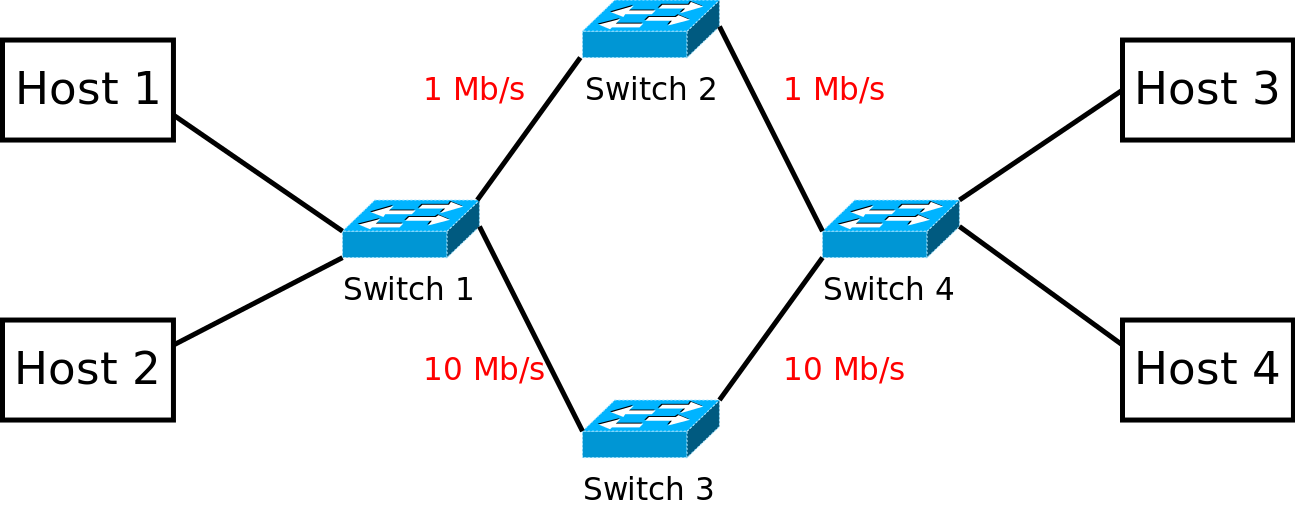
\includegraphics[width=\linewidth]{imagenes/Environment/mininet_topology.png}
  \caption{Base Mininet topology.}
  \label{fig:mininet_topology}
\end{figure}

Once we know what topology we want to create, we will use Mininet's Python API to build it. Alternatively, there is a GUI application called MiniEdit used to create a Mininet network in a visual way. Despite MiniEdit being the easier option, we will opt for the Python API because we would like to take a lower level approach. The code can be found at Appendix \ref{annex:mininet}.

To simplify the CLI command used to invoke the topology, we will place the Python file under /home/mininet/mininet/custom/.

Lastly, to build the network we use the command:
\begin{lstlisting}
    $ sudo mn --custom ~/onstutorial/flowvisor_scripts/<python filename> --topo <topology name> --link tc --controller remote --mac
\end{lstlisting}

Some of the flags used on the command above are not required to build our custom network, but they will be necessary for the testing process.
\begin{enumerate}
    \item \textbf{- -link tc}. Enables link bandwidth customization.
    \item \textbf{- -controller remote}. Will allow us to, later on, connect the network to FlowVisor.
    \item \textbf{- -mac}. (Optional). Disables MAC randomization for each host and makes it easier to associate each MAC to its correspondent host. This is very helpful for debugging.
\end{enumerate}

\subsection{Enabling External Hosts}
To prepare the topology for the coming tests, we have to adjust the network so that it can handle two external interfaces, Figure \ref{fig:mininet_topology_external}. This is where the Mininet CLI falls short. These external interfaces have to be added after the topology is created, which is not possible through the CLI. Therefore, we have to use the Python API for both creating the topology and running it.

\begin{figure}
  \centering
  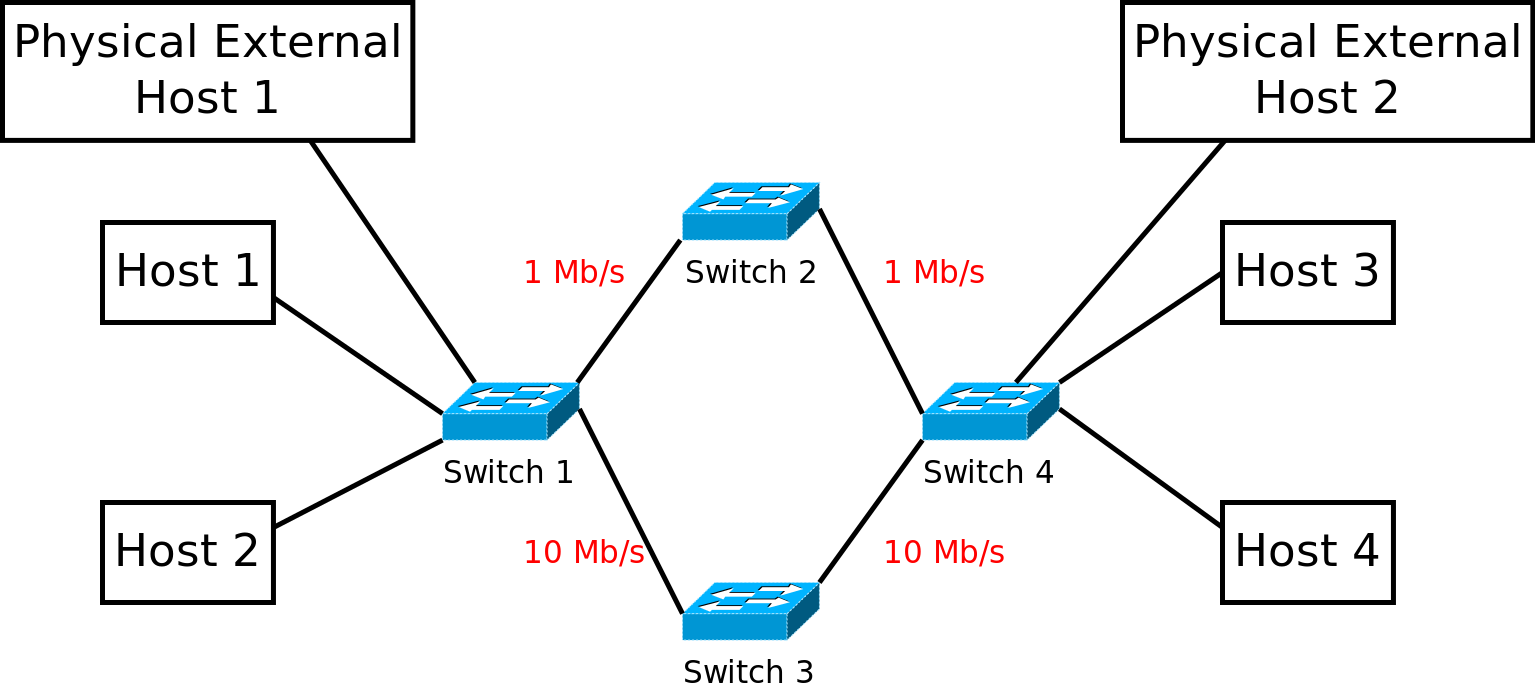
\includegraphics[width=\linewidth]{imagenes/Environment/mininet_topology_external_hosts.png}
  \caption{Mininet topology with added external hosts.}
  \label{fig:mininet_topology_external}
\end{figure}

Once the logic for running the network is added to the Python file, we no longer need to use the command line. We can launch the network by calling the Python file directly.
\begin{lstlisting}
    $ sudo python <python filename>
\end{lstlisting}

With the external interfaces added, our topology is almost ready to start handling some traffic. We are only lacking one element, although a very important one, a controller. An SDN becomes almost useless without a controller. However, an explanation on how to set up the controllers after can be found in the next chapter. 

\subsection{IP Address Assignment}
Finally, it is important to assign IP addresses correctly for the network to work correctly. We will not implement router functionality and as a result, hosts that want to communicate with each other must be assigned to the same sub network. IP assignments are shown in Tables \ref{tab:IP_virtual_hosts} and \ref{tab:IP_external_hosts} for virtual and physical hosts respectively. Since each host only has one available port, we will omit it.

\begin{table}
    \centering
    \caption{IP and MAC Addresses for the virtual hosts.}
    \vspace{0.1 cm}
    \begin{tabular}{c c c c}
    \hline
    \rowcolor{lightgray}
    \textbf{Virtual Host}               &\textbf{IPv4 Address} &\textbf{Network Mask}   &\textbf{MAC Address}     \\ \hline
    Host 1                              &  10.0.0.1            & 255.255.0.0            & 00:00:00:00:00:01       \\ \hline 
    Host 2                              &  192.168.0.2         & 255.255.0.0            & 00:00:00:00:00:02       \\ \hline 
    Host 3                              &  10.0.0.3            & 255.255.0.0            & 00:00:00:00:00:03       \\ \hline 
    Host 4                              &  192.168.0.4         & 255.255.0.0            & 00:00:00:00:00:04       \\ \hline 
    \end{tabular}
    \label{tab:IP_virtual_hosts}
\end{table}

\begin{table}
    \centering
    \caption{IP and MAC addresses for the physical hosts.}
    \vspace{0.1 cm}
    \begin{tabular}{c c c c}
    \hline
    \rowcolor{lightgray}
    \textbf{Physical Host}              &\textbf{IPv4 Address}     &\textbf{Network Mask}   &\textbf{MAC Address}     \\ \hline
    Host 1                              &  192.168.100.1           & 255.255.0.0            & 00:00:00:00:00:01       \\ \hline 
    Host 2                              &  192.168.100.101         & 255.255.0.0            & 00:00:00:00:00:02       \\ \hline 
    \end{tabular}
    \label{tab:IP_external_hosts}
\end{table}

Regarding the virtual switches, we need some kind of identifier to refer to them when configuring FlowVisor. This identifier is called DPID. To make it easier to identify each virtual switch, we have assigned the DPID manually during the creation of the network, Table \ref{tab:DPID_assignment}.

\begin{table}
    \centering
    \caption{DPID for each virtual switch.}
    \vspace{0.1 cm}
    \begin{tabular}{c c}
    \hline
    \rowcolor{lightgray}
    \textbf{Virtual Switch}              &\textbf{DPID}            \\ \hline
    Switch 1                             & 00:00:00:00:00:01       \\ \hline 
    Switch 2                             & 00:00:00:00:00:02       \\ \hline 
    Switch 3                             & 00:00:00:00:00:03       \\ \hline 
    Switch 4                             & 00:00:00:00:00:04       \\ \hline 
    \end{tabular}
    \label{tab:DPID_assignment}
\end{table}

We are now ready to implement FlowVisor on top of our network and start commence the slicing.